\begin{center}
    \Large{\textbf{第六、八章作业及小测解答}}
\end{center}

第六章“自旋与全同粒子体系”对应曾谨言书上第九章
\begin{enumerate}[label=\textbf{6.\arabic*}, listparindent=\parindent]

\setcounter{enumi}{1}
\item
{\color{red}\textbf{讨论:}}

本题还可以用作业3.22(即《解答》5.10)中“旋转”的观点去理解。在$\sigma_z$表象中,$\sigma_z$本征态写作$\psi_{\frac{1}{2}}=\smqty(1\\0)$, $\psi_{-\frac{1}{2}}=\smqty(0\\1)$。将$\vec{e}_z$方向转至$\vec{n}=(\sin\theta\cos\varphi,\sin\theta\sin\varphi,\cos\theta)$,可先沿着$y$轴转$\theta$角,再沿着$z$轴转$\varphi$角。因此根据作业3.22可知$\vec{\sigma\cdot n}$
的本征态为
\[\phi_{\pm\frac{1}{2}}=\ee{-\im\hat{s}_z\varphi/\hbar}\,\ee{-\im\hat{s}_y\theta/\hbar}\,\psi_{\pm\frac{1}{2}}\]
这个公式首先是用自旋$\frac{1}{2}$的角动量算符$\hat{\vec{s}}$写出的。我们知道$\hat{\vec{s}}=\frac{\hbar}{2}\vec{\sigma}$。又因为有
\[\ee{\im\lambda\vec{\sigma\cdot n}} =\cos\lambda + \im\sin\lambda(\vec{\sigma\cdot n})\]
(注意这是对自旋$\frac{1}{2}$特有的公式。)所以
\alg{\ee{-\im\hat{s}_z\varphi/\hbar}\,\ee{-\im\hat{s}_y\theta/\hbar} 
= \ee{-\im\frac{\varphi}{2}\sigma_z}\,\ee{-\im\frac{\theta}{2}\sigma_y}= \mqty(\ee{-\im\frac{\varphi}{2}} & \\ & \ee{\im\frac{\varphi}{2}})
\mqty(\cos\frac{\theta}{2} & -\sin\frac{\theta}{2}\\ \sin\frac{\theta}{2}&\cos\frac{\theta}{2})= \mqty(\cos\frac{\theta}{2}\ee{-\im\frac{\varphi}{2}} & -\sin\frac{\theta}{2}\ee{-\im\frac{\varphi}{2}}\\ \sin\frac{\theta}{2}\ee{\im\frac{\varphi}{2}}&\cos\frac{\theta}{2}\ee{\im\frac{\varphi}{2}})}
将其作用在$\psi_{\pm\frac{1}{2}}$上有
\[\phi_{\frac{1}{2}}=\mqty(\cos\frac{\theta}{2}\ee{-\im\frac{\varphi}{2}} \\ \sin\frac{\theta}{2}\ee{\im\frac{\varphi}{2}}),\quad \phi_{-\frac{1}{2}}=\mqty(-\sin\frac{\theta}{2}\ee{-\im\frac{\varphi}{2}}\\\cos\frac{\theta}{2}\ee{\im\frac{\varphi}{2}})\]
也可以验证$\sigma_z$的变换(注意$\sigma_z$右边e指数的顺序)
\alg{\ee{-\im\frac{\varphi}{2}\sigma_z}\,\ee{-\im\frac{\theta}{2}\sigma_y}\,\sigma_z\,\ee{\im\frac{\theta}{2}\sigma_y}\,\ee{\im\frac{\varphi}{2}\sigma_z}
&= \mqty(\cos\frac{\theta}{2}\ee{-\im\frac{\varphi}{2}} & -\sin\frac{\theta}{2}\ee{-\im\frac{\varphi}{2}}\\ \sin\frac{\theta}{2}\ee{\im\frac{\varphi}{2}}&\cos\frac{\theta}{2}\ee{\im\frac{\varphi}{2}})
\mqty(1&\\&-1)
\mqty(\cos\frac{\theta}{2}\ee{\im\frac{\varphi}{2}} & \sin\frac{\theta}{2}\ee{-\im\frac{\varphi}{2}}\\ -\sin\frac{\theta}{2}\ee{\im\frac{\varphi}{2}}&\cos\frac{\theta}{2}\ee{-\im\frac{\varphi}{2}})\\
&= \mqty(\cos\theta & \sin\theta\ee{-\im\varphi}\\ \sin\theta\ee{\im\varphi} & -\cos\theta) = \vec{\sigma\cdot n}}
请同学们自行验算上面的式子。

\setcounter{enumi}{4}
\item
【另解】

\noindent(b) 可直接利用$V_T(r)S_{12} = V_T(r)\,(6S_n^2-2\vec{S}^2)$以及对$\vec{S}$的自旋单态有
\[S_n\ket{\psi;00} = 0,\quad \vec{S}\ket{\psi;00}=0\]
因此张量势$V_T(r)S_{12}\ket{\psi;00}\equiv 0$,
故张量力恒为0。

\setcounter{enumi}{11}
\item
{\color{red}\textbf{讨论:}}

可以继续6.2题对一般的角动量旋转做一讨论,对任意角动量算符$\hl$ (满足$[\hat{l}_i,\hat{l}_j]=\im\eijk\hat{l}_k$),有
\[\ee{-\im\theta \vec{n\cdot }\hat{\vec{l}}/\hbar}\,(\vnt\vec{\cdot}\hl)\,\ee{\im\theta \vec{n\cdot}\hat{\vec{l}}/\hbar} = \vnt'\vec{\cdot}\hl\]
解读为沿$\vnt$方向的角动量 (即$\vnt\vec{\cdot}\hl$) 经旋转后变成沿$\vnt'$方向的角动量,$\vnt'$单位矢量是将$\vnt$以$\vec{n}$为转轴逆时针旋转$\theta$角后得到的。根据几何知识,将$\vnt$在$\vec{n}$上投影大小为$\vn\vec{\cdot}\vnt$,在其法平面上投影(矢量)为$(\vn\vec{\times}\vnt)\vec{\times}\vn$,法平面上与之垂直等大的矢量为$\vn\vec{\times}\vnt$ (还需注意有前后两个方向),故
\[\vn_l'=(\vn\vec{\cdot}\vnt)\vn+\qty((\vn\vec{\times}\vnt)\vec{\times}\vn)\cos\theta + (\vn\vec{\times}\vnt)\sin\theta\]
在本章处理的$\frac{1}{2}$自旋中,$\hl=\frac{\hbar}{2}\vec{\sigma}$,$\ee{\im\lambda\vec{n\cdot\sigma}} = \ee{\im(2\lambda)\vec{n\cdot }\hl/\hbar}$,因此对本题而言,最直接的等式是
\[\ee{\im\lambda \vec{n\cdot\sigma}}\,(\vnt\vec{\cdot\sigma})\,\ee{-\im\lambda \vec{n\cdot\sigma}} = \qty[(\vn\vec{\cdot}\vnt)\vn+\qty((\vn\vec{\times}\vnt)\vec{\times}\vn)\cos(-2\lambda) + (\vn\vec{\times}\vnt)\sin(-2\lambda)]\vec{\cdot \sigma}\]
如何将该式化为题中的式子?容易利用爱因斯坦记号展开证明以下恒等式
\[(\vA\btimes\vB)\bcdot\vC = -(\vA\btimes\vC)\bcdot\vB,\quad\qty[(\vA\btimes\vB)\btimes\vC]\bcdot\vD = \qty[(\vA\btimes\vD)\btimes\vC]\bcdot\vB\]
因此可将右式的$\vec{\sigma}$与$\vnt$交换,并改变第三项的符号。两边同时约去$(\vnt\bcdot)$即为题中要证的式子。

\setcounter{enumi}{22}
\item
{\color{red}\textbf{讨论:}}

此类问题都可以用6.24解法二的方法,分$j=l\pm\frac{1}{2}$两类情况分别计算结果。前提是牢记非耦合表象$(\vec{l}^2,m_l,m_s)$本征态到耦合表象$(\vec{l}^2,\vec{j}^2,m_j)$本征态的变换系数:
\[\ket{l,j=l+\tfrac{1}{2},m_j}=\mqty(\sqrt{\frac{l+m+1}{2l+1}}\Y_{lm}\\\sqrt{\frac{l-m}{2l+1}}\Y_{l,m+1}),\quad
\ket{l,j=l-\tfrac{1}{2},m_j}=\mqty(-\sqrt{\frac{l-m}{2l+1}}\Y_{lm}\\\sqrt{\frac{l+m+1}{2l+1}}\Y_{l,m+1})
\]
请大家练习直接用上式推导本题结果。

\setcounter{enumi}{30}
\item

\noindent (1) 设单位径矢量$\hr=(\sin\theta\cos\varphi,\,\sin\theta\sin\varphi,\,\cos\theta)$,则 
\[h=\frac{1}{2}\mqty(\cos\theta & \sin\theta\ee{-\im\varphi}\\ \sin\theta\ee{\im\varphi} & -\cos\theta)\]
之后参见6.2题。

\noindent (2) 根据$\ee{\im\lambda\vec{\sigma\cdot n}} =\cos\lambda + \im\sin\lambda(\vec{\sigma\cdot n})$,代入$\lambda=\frac{\pi}{2}$:
\[\ee{\im\pi h}=\ee{-\im\frac{\pi}{2}\vec{\sigma\cdot n}}=\cos\frac{\pi}{2}+\im(2h)\sin\frac{\pi}{2}=2\im h\]

\noindent (3) 由$h^2=\frac{1}{4}$可知$h^{-1}=4h$,
\[\tilde{F}=U^{-1}FU=h^{-1}F h=4hFh\]
而
\[F+4h\,[F,\,h] = F+4hFh-4h^2F = F+4hFh-F = 4hFh\]
两式相等.

\noindent (4) 用爱因斯坦符号推导最为方便。以下用$\vec{n}$代替单位径矢,$\vec{n}=(n_x,n_y,n_z)$。{\color{red}推导中最常用的两个式子是:}
\alg{&\sigma_i\sigma_j = \delta_{ij}+\im\eijk\sigma_k\quad\text{(用于减少$\sigma$的个数。最后每项只含0或1个$\sigma$)}\\
&\eijk\varepsilon_{ijl} = 2\,\delta_{kl},\quad\varepsilon_{ijk}\varepsilon_{ilm} = \delta_{jl}\delta_{km}-\delta_{jm}\delta_{kl},\quad\text{(用于所并两个$\varepsilon$)}}
总结一下基本思想:用第一行等式不断减少$\sigma$个数,但会增加$\varepsilon$,随后用第二行等式将两个$\varepsilon$缩并进行化简。遇到有$l$的项需想办法构造对易式(如$[l_i,\,n_j]$, $[l_i,\,\sigma_jn_j]$等)将其去除。
\begin{enumerate}
    \item 计算$\tilde{\vec{s}}$。我们以$\tilde{\vec{s}}=4h\vec{s}h = \frac{1}{2}(\vec{\sigma\cdot n})\,\vec{\sigma}\,(\vec{\sigma\cdot n })$为出发点,
    考虑其$i$分量(\,{\color{red}\underline{下划线}}表示每一步推导要点):
    \alg{\tilde{s}_i=\tfrac{1}{2}(\underline{\sigma_j}n_j)\,\underline{\sigma_i}\,(\sigma_l n_l)&=\tfrac{1}{2}(\delta_{ij}-\im\eijk\underline{\sigma_k})\,\underline{\sigma_l}n_jn_l\\
    &= \tfrac{1}{2}n_i\sigma_ln_l - \tfrac{1}{2}\im\underline{\eijk}(\delta_{kl}+\im\underline{\eklm}\sigma_m)n_jn_l\\
    &= \tfrac{1}{2}n_i\sigma_ln_l - \tfrac{1}{2}\im\eijk n_jn_k+\tfrac{1}{2}(\delta_{il}\delta_{jm}-\delta_{im}\delta_{jl})\sigma_mn_jn_l\\
    &= \tfrac{1}{2}n_i\sigma_ln_l-0 +\tfrac{1}{2}\sigma_jn_jn_i - \tfrac{1}{2}\sigma_in_jn_j\\
    &= n_i\sigma_j n_j - \tfrac{1}{2}\sigma_i = \qty[\vec{n}\,(\vec{\sigma\cdot}\hr)-\tfrac{1}{2}\vec{\sigma}]_i}
    因此$\tilde{\vec{s}}=-\vec{s}+2\,\vn h$.
    
    \item 计算$\tilde{\vec{l}}$。首先,
    \alg{[l_i,\,n_j]&=[l_i,\,\tfrac{r_j}{r}]=[l_i,\,r_j]\,\tfrac{1}{r}+r_j\,[l_i,\,\tfrac{1}{r}]=\im\eijk r_k\tfrac{1}{r}+0=\im\eijk n_k\\   [l_i,\,\vec{\sigma\cdot n}]&=\qty[l_i,\,\sigma_jn_j] = [l_i,\sigma_j]\,n_j+\sigma_j\,[l_i,\,n_j]= 0+\sigma_j\im\eijk n_k = \im\eijk \sigma_jn_k}
    用(3)问的结论:
    \alg{\tilde{l}_i=l_i+(\vec{\sigma\cdot n})\,[l_i,\,\vec{\sigma\cdot n}]
    &= l_i+\underline{\sigma_l} n_l\,(\im\eijk\underline{\sigma_j} n_k) \\
    &= l_i+\im\underline{\eijk}\,(\delta_{jl}+\im\underline{\varepsilon_{ljm}}\sigma_m)n_ln_k\\
    &= l_i+\im\eijk n_j n_k - (\delta_{km}\delta_{il}-\delta_{kl}\delta_{im})\,\sigma_m n_l n_k\\
    &= l_i +0 -\sigma_kn_in_k+\sigma_in_kn_k = l_i-n_i\,(\vec{\sigma\cdot n})+\sigma_i}
    最后一步用到$n_kn_k=1$。因此$\tilde{\vec{l}}=\vec{l}-2\,\vec{n}h+2\vec{s}$.
    \item 计算$\tilde{\vec{j}}$。
    \[\tilde{\vec{j}}=\tilde{\vec{l}}+\tilde{\vec{s}}= \vec{l}-2\,\vec{n}h+2\vec{s}-\vec{s}+2\,\vn h =\vec{l}+\vec{s}= \vec{j}\]
    说明$[\vec{j},\,h]=0$.
    若直接推导:
    \[[j_i,\,\vec{\sigma\cdot n}]=[l_i,\,\vec{\sigma\cdot n}]+\tfrac{1}{2}[\sigma_i,\,\sigma_jn_j]=\im\eijk\sigma_jn_k+\tfrac{1}{2}(2\im\eijk\sigma_k)n_j = 0\]
    
    \item 计算$\tilde{\vec{l}}^2$。{\color{red}请注意题目答案有误。}我们提供三种解法,前两种善用前面小问的结果,稍显简洁;第三种暴力求解。
    
    【法一】
    直接对(b)结果进行平方:$\tilde{\vec{l}}^2=(\tilde{\vec{l}})^2=(l_i+\sigma_i-n_i\sigma_kn_k)(l_i+\sigma_i-n_i\sigma_ln_l)$。注意爱因斯坦记号要求每个下表必须只能出现1或2次, 2次代表指标缩并,出现多于2次是违规的。故上面用了$k$和$l$两组下标。
    展开为
    \[\tilde{\vec{l}}^2 = l_il_i+\sigma_i\sigma_i+ n_in_i\sigma_kn_k\sigma_ln_l+
    2\,l_i\sigma_i-2\,l_in_i\sigma_kn_k - 2\,\sigma_in_i\sigma_kn_k \]
    上式代入
    \[l_in_i=0,\quad \sigma_i\sigma_i = 3,\quad\sigma_in_i\sigma_jn_j=(\vec{\sigma\cdot n})^2=1\]
    得到$\tilde{\vec{l}}^2=l_il_i+3+1+2\,l_i\sigma_i-0-2 = \vec{l}^2+4\,(\vec{s\cdot l})+2$.
    
    【法二】善用(b)的结果。将所求化为
    \alg{\tilde{\vec{l}}^2=\vec{l}^2+(\vec{\sigma\cdot n})\,[\vec{l}^2,\,\vec{\sigma\cdot n}] &= \vec{l}^2+\underline{(\vec{\sigma\cdot n})}\,\underline{l_i}\,[l_i,\,\vec{\sigma\cdot n}]+(\vec{\sigma\cdot n})\,[l_i,\,\vec{\sigma\cdot n}]\,l_i\\
    &= \vec{l}^2+l_i\,(\vec{\sigma\cdot n})\,[l_i,\,\vec{\sigma\cdot n}]-[l_i,\,\vec{\sigma\cdot n}][l_i,\,\vec{\sigma\cdot n}]+(\vec{\sigma\cdot n})\,[l_i,\,\vec{\sigma\cdot n}]\,l_i}
    由(b)知$(\vec{\sigma\cdot n})[l_i,\,\vec{\sigma\cdot n}]=\sigma_i+n_i\sigma_kn_k$,且$[l_i,\,\vec{\sigma\cdot n}]=\im\eijk\sigma_jn_k$,代入有
    \alg{\tilde{\vec{l}}^2 &=\vec{l}^2+l_i\,(\sigma_i+n_i\sigma_kn_k)-(\im\underline{\eijk}\sigma_jn_k)(\im\underline{\varepsilon_{ilm}}\sigma_ln_m)+(\sigma_i+n_i\sigma_kn_k)\,l_i\\
    &= \vec{l}^2+(l_i\sigma_i+0)-\qty(-(\delta_{jl}\delta_{km}-\delta_{jm}\delta_{kl})\,\sigma_j\sigma_ln_kn_m)+(\sigma_il_i+0)\\
    &= \vec{l}^2+l_i\sigma_i+(\sigma_j\sigma_jn_kn_k-\sigma_jn_k\sigma_k\sigma_j)+l_i\sigma_i\\
    &= \vec{l}^2+l_i\sigma_i+(3-1)+l_i\sigma_i }
    故$\tilde{\vec{l}}^2= \vec{l}^2+4\,(\vec{s\cdot l})+2$。
    
    【法三】暴力求解。
    从$\tilde{\vec{l}}^2=\vec{l}^2+(\vec{\sigma\cdot n})\,[\vec{l}^2,\,\vec{\sigma\cdot n}]$出发,首先\;{\color{red} (注意到$l$和$\sigma$可交换,但$l$和$n$不可交换!)}
    \alg{[\vec{l}^2,\,\vec{\sigma\cdot n}]=[l_il_i,\,\sigma_jn_j] &= l_i\,[l_i,\,\sigma_jn_j]+[l_i,\,\sigma_jn_j]\,l_i = \im\eijk\sigma_j (l_in_k+n_kl_i) \\
    &= 2\im\eijk\sigma_j n_kl_i + \im\eijk\sigma_j\,[l_i,n_k]\\
    &= 2\im\eijk\sigma_j n_kl_i + \im\underline{\eijk}\sigma_j\,(\im\underline{\varepsilon_{ikl}}n_l)\\
    &= 2\im\eijk\sigma_j n_kl_i -(-2\,\delta_{jl}\sigma_jn_l) = 2\im\eijk\sigma_j n_kl_i+2\,\sigma_jn_j}
    因此
    \alg{\tilde{\vec{l}}^2 &= \vec{l}^2+(\underline{\sigma_l}n_l)\,\qty(2\im\eijk\underline{\sigma_j} n_kl_i+2\,\sigma_jn_j) \\
    &= \vec{l}^2+(\delta_{lj}+\im\underline{\varepsilon_{ljm}}\sigma_m)\,2\im\,\underline{\eijk} n_ln_kl_i + 2\,\sigma_ln_l\sigma_jn_j\\
    &= \vec{l}^2+2\im\,\eijk n_jn_kl_i -2\,(\delta_{km}\delta_{il}-\delta_{kl}\delta_{im})\,\sigma_mn_ln_kl_i+2\,\sigma_ln_l\sigma_jn_j\\
    &= \vec{l}^2+2\im\,\eijk n_jn_kl_i - 2\,\sigma_kn_in_kl_i + 2\,\sigma_in_kn_kl_i + 2\,\sigma_ln_l\sigma_jn_j}
    上式第二项$i,j$反称故为0;第三项交换$n_in_k$后因为有$n_il_i=\eijk r_ir_jp_k/r = 0$ (经典上理解:$\vec{n\cdot l}=0$, 同理也可证$l_in_i=0$)故为0。因此
    $\tilde{\vec{l}}^2 = \vec{l}^2+2\,\sigma_il_i+2=\vec{l}^2+4\,(\vec{s\cdot l})+2$即为所求.
    
    \item 求$\tilde{\vec{l}}\bcdot\tilde{\vec{s}}$。
    
    【法一】直接将(a), (b)结果相乘。有
    \alg{\tilde{l}_i\tilde{s}_i &= (l_i+\sigma_i-n_i\sigma_jn_j)(n_i\sigma_kn_k - \tfrac{1}{2}\sigma_i)\\
    &= (l_in_i\sigma_kn_k + \sigma_in_i\sigma_kn_k - n_in_i\sigma_jn_j\sigma_kn_k) + (-\tfrac{1}{2}l_i\sigma_i-\tfrac{1}{2}\sigma_i\sigma_i + \tfrac{1}{2}\sigma_in_i\sigma_jn_j)\\
    &= (0+1-1)+(-\tfrac{1}{2}l_i\sigma_i-\tfrac{3}{2}+\tfrac{1}{2}) = -\tfrac{1}{2}l_i\sigma_i-1}
    故$\tilde{\vec{l}}\bcdot\tilde{\vec{s}} = -\vec{l\cdot s}-1$.
    
    【法二】【法三】 可以用类似于(d)问的法二、法三的思想进行求解,请同学们自己练习推导。
\end{enumerate}
{\color{red}\textbf{注:}此题算错的同学很多,绝大多数同学没有发现答案有误。助教批改的不仔细,还请大家自己核查一遍过程。其中最容易出错的地方就是直接交换$l$和$n$算符,答案的失误似也与之有关。}

\end{enumerate}

第八章“电磁场中的粒子”对应曾谨言书上第七章
\begin{enumerate}[label=\textbf{8.\arabic*}, listparindent=\parindent]

\setcounter{enumi}{1}
\item
{\color{red}\textbf{注:}}恒磁场中粒子运动的朗道能级的求解还需掌握{\color{red}能级简并的特征}。请大家复习下这一部分内容。


\end{enumerate}

小测题目解答:
\begin{enumerate}[label=\textbf{6.\Alph*}, listparindent=\parindent]

\item 
\begin{enumerate}[listparindent=\parindent]
\item \emph{推导:$\ee{\im\theta \vec{\sigma\cdot n}}=\cos\theta+\im\sin\theta\vec{\sigma\cdot n}$.}

进行幂级数展开
\alg{\ee{\im\theta\vec{\sigma\cdot n}}=\sum_{n=0}^{\infty}\frac{1}{n!}(\im\theta\vec{\sigma\cdot n})^n}
由于
\[(\vec{\sigma\cdot n})^2 = \sigma_in_i\sigma_j n_j = (\delta_{ij}+\im\eijk\sigma_k)\,n_in_j = \delta_{ij}n_in_j = 1\]
故\[(\vec{\sigma\cdot n})^{2k}=1,\quad(\vec{\sigma\cdot n})^{2k+1}=\vec{\sigma\cdot n},\quad \text{$k$为整数}\]
\[\ee{\im\theta\vec{\sigma\cdot n}}=\sum_{k=0}^{\infty}\frac{1}{(2k)!}(-\im\theta)^{2k}+\sum_{k=0}^{\infty}\frac{1}{(2k+1)!}(-\im\theta)^{2k+1}(\vec{\sigma\cdot n})=\cos\theta + \im\sin\theta\,\vec{\sigma\cdot n}\]
证毕。

\item \emph{推导:$\Tr((\vec{\sigma\cdot A})(\vec{\sigma\cdot B})(\vec{\sigma\cdot C})) = 2\im\,(\vec{A\times B})\bcdot\vec{C}$,其中$\vA$, $\vB$, $\vC$为矢量.}

我们知道$(\vec{\sigma\cdot n})^2=1$,故无论多么复杂的$\vec{\sigma}$矩阵表达式都可以最终化为$A_0+B_0\,\vec{\sigma\cdot n}_0$的形式。这也可以从爱因斯坦记号的表示看出:因为有$\sigma_i\sigma_j=\delta_{ij}+\im\eijk\sigma_k$,总可以将两个$\sigma$缩并以减少1个$\sigma$矩阵,使得最后的每一项中都不含$\sigma$或只含1个$\sigma$矩阵。

为此可以将$\Tr(\cdot)$内部矩阵化简(下划线表示推导要点)
\alg{(\vec{\sigma\cdot A})(\vec{\sigma\cdot B})(\vec{\sigma\cdot C})&=\underline{\sigma_i}A_i\underline{\sigma_j}B_j\sigma_kC_k = (\delta_{ij}+\im\varepsilon_{ijl}\underline{\sigma_l})\underline{\sigma_k}A_iB_jC_k\\
&= \sigma_kA_iB_iC_k + \im\underline{\varepsilon_{ijl}}(\delta_{lk}+\im\underline{\varepsilon_{lkm}}\sigma_m)A_iB_jC_k\\
&= \sigma_kA_iB_iC_k + \im\varepsilon_{ijk}A_iB_jC_k - (\delta_{ik}\delta_{jm}-\delta_{im}\delta_{jk})\sigma_mA_iB_jC_k\\
&= \sigma_kA_iB_iC_k + \im\varepsilon_{ijk}A_iB_jC_k -\sigma_jA_iB_jC_i + \sigma_iA_iB_jC_j}
现在结果中每一项都含0个或1个$\sigma$。由于
\[\Tr(I)=2,\quad \Tr(\sigma_i)=0,\]
则只有不含$\sigma$项对矩阵的迹有贡献:\[\Tr((\vec{\sigma\cdot A})(\vec{\sigma\cdot B})(\vec{\sigma\cdot C}))=2\im\varepsilon_{ijk}A_iB_jC_k=2\im\,(\vec{A\times B})\bcdot\vec{C}.\]

\item \emph{化简:$\ee{\im\theta\vec{\sigma\cdot n}}\,(\vec{l\cdot \sigma})\,\ee{-\im\theta\vec{\sigma\cdot n}}$, 其中$\vec{n}=\frac{\vec{r}}{r}$为单位径向矢量,$\vec{l}$为轨道角动量.}

显然本题与6.12题很像。根据我们对6.12的几何诠释,相当于沿$\vec{l}$方向的自旋算符绕$\vec{n}$旋转。由于本题中$\vec{l}$方向是与$\vec{n}$垂直的,故不存在沿$\vn$方向的投影,问题还可以进一步简化。一个直接的想法是对6.12题结论等式两边点乘$\vec{l}$即可。但是,$\vec{l}$并不是普通矢量,它与$\vec{n}$是不对易的,满足
\[[l_i,\,n_j]=\im\varepsilon_{ijk}n_k.\]
故我们先将原式化为
\[\ee{\im\theta\vec{\sigma\cdot n}}\,l_i\sigma_i\,\ee{-\im\theta\vec{\sigma\cdot n}} = l_i\qty(\ee{\im\theta\vec{\sigma\cdot n}}\,\sigma_i\,\ee{-\im\theta\vec{\sigma\cdot n}})-[l_i,\,\ee{\im\theta\vec{\sigma\cdot n}}]\,\sigma_i\,\ee{-\im\theta\vec{\sigma\cdot n}}\]
第一项则回到6.12题的方法中来,可以得出 (请同学们补全过程)
\[l_i\qty(\ee{\im\theta\vec{\sigma\cdot n}}\,\sigma_i\,\ee{-\im\theta\vec{\sigma\cdot n}}) = l_i\sigma_i\,\cos2\theta +\eijk l_in_j\sigma_k\,\sin2\theta=(\vec{l\cdot \sigma})\cos2\theta+\vec{l}\bcdot(\vec{n\times\sigma})\,\sin2\theta\]

下面求第二项。首先求解对易关系
\[[l_i,\,\ee{\im\theta\sigma_jn_j}]=[l_i,\,\im\sin\theta\sigma_jn_j]=\im\sin\theta\,(\im\eijk \sigma_j n_k)\]
故
\alg{[l_i,\,\ee{\im\theta\sigma_jn_j}]\,\sigma_i &= -\sin\theta\,\eijk\underline{\sigma_j} n_k \underline{\sigma_i}\\
&= -\sin\theta\,\underline{\eijk}\,(\delta_{ij}-\im\underline{\varepsilon_{ijl}}\sigma_l)\,n_k \\
&= \im\sin\theta\,(2\delta_{kl})\,\sigma_ln_k=2\im\sin\theta\sigma_kn_k}
最后
\alg{[l_i,\,\ee{\im\theta\sigma_jn_j}]\,\sigma_i\,\ee{-\im\theta\sigma_ln_l}
&=2\im\sin\theta\,\sigma_kn_k\,(\cos\theta-\im\sin\theta\,\sigma_ln_l) \\
&= \im\,(\vec{n\cdot\sigma})\,\sin2\theta+2\sin^2\theta}
\end{enumerate}
最终结果为
\alg{\ee{\im\theta\vec{\sigma\cdot n}}\,l_i\sigma_i\,\ee{-\im\theta\vec{\sigma\cdot n}}&=
(\vec{l\cdot \sigma})\cos2\theta+\vec{l}\bcdot(\vec{n\times\sigma})\,\sin2\theta -\im\,(\vec{n\cdot\sigma})\,\sin2\theta-2\sin^2\theta\\
&= 
(\vec{l\cdot \sigma}+1)\,\cos2\theta+[\vec{l}\bcdot(\vec{n\times\sigma})-\im\,(\vec{n\cdot\sigma})]\,\sin2\theta-1.}


\noindent【法二】
可使用定理
\[\ee{A}\,B\,\ee{-A}=B+[A,B]+\frac{1}{2!}\qty[A,\,[A,B]]+\cdots\]
首先看看6.12题在本方法下的表现如何。可以归纳地证明 (通过算前几阶先找到规律):
\alg{&\Big[\underbrace{\im\theta\sigma_{j'}n_{j'},\cdots,[\im\theta\sigma_jn_j}_{\text{$2m+1$层}},\,\sigma_i]\Big]=(2\theta)^{2m+1}(-1)^{m}\,\varepsilon_{ijk}n_j\sigma_k,\quad&m=0,1,2,\cdots\\
&\Big[\underbrace{\im\theta\sigma_{j'}n_{j'},\cdots,[\im\theta\sigma_jn_j}_{\text{$2m$层}},\,\sigma_i]\Big]=(2\theta)^{2m}(-1)^{m}\,(\sigma_i-n_i\sigma_kn_k ),\quad&m=1,2,3,\cdots}
第0阶是一个例外,它显然等于$\sigma_i$。由此可以得到
\alg{\ee{\im\theta\vec{\sigma\cdot n}}\,\sigma_i\,\ee{-\im\theta\vec{\sigma\cdot n}}
&=(\sigma_i-n_i\sigma_kn_k )\,\cos2\theta + \varepsilon_{ijk}n_j\sigma_k\,\sin2\theta + n_i\sigma_kn_k\\
&=[(\vec{n\times\sigma})\btimes\vec{n}]_i\,\cos2\theta+(\vec{n\times\sigma})_i\,\sin2\theta+n_i(\vec{\sigma\cdot n})
}
最后一项正是为了补偿第0阶而加上的常数。可以验证这正是6.12的结果。

对于本例,用$l_i\sigma_i$替代$\sigma_i$,发现$l_i$会参与到对易关系当中。有
\alg{&\Big[\underbrace{\im\theta\sigma_{j'}n_{j'},\cdots,[\im\theta\sigma_jn_j}_{\text{$2m+1$层}},\,\sigma_i]\Big]=(2\theta)^{2m+1}(-1)^{m}\,(l_i\varepsilon_{ijk}n_j\sigma_k-\im\sigma_kn_k),\quad&m=0,1,2,\cdots\\
&\Big[\underbrace{\im\theta\sigma_{j'}n_{j'},\cdots,[\im\theta\sigma_jn_j}_{\text{$2m$层}},\,\sigma_i]\Big]=(2\theta)^{2m}(-1)^{m}\,(l_i\sigma_i-l_in_i\sigma_kn_k +1),\quad&m=1,2,3,\cdots}
可见两式各多出了最后一项,这是由于$l_i$参与对易关系带来的。当然第0阶仍是例外,它应等于$l_i\sigma_i$。再利用$l_in_i=0$将第2式第二项去掉,可以得到
\[\ee{\im\theta\vec{\sigma\cdot n}}\,l_i\sigma_i\,\ee{-\im\theta\vec{\sigma\cdot n}}=
(\vec{l\cdot \sigma}+1)\,\cos2\theta+[\vec{l}\bcdot(\vec{n\times\sigma})-\im\,(\vec{n\cdot\sigma})]\,\sin2\theta-1.\]

\item \emph{类氢原子的价电子处于$l=1$的态上,置于均匀磁场$\vec{B}=B\,\vec{e}_z$中。哈密顿量可表为(近似地)
\[\hH=\frac{\mu_BB}{\hbar}(\hat{L}_z+2\hat{S}_z)+\frac{2w}{\hbar^2}\hat{\vec{L}}\bcdot\hat{\vec{S}},\]
其中$w$为常数。$\hat{L}_z$的三个本征态为$\varphi_1$, $\varphi_0$, $\varphi_{-1}$; $\hat{S}_z$的本征函数为$\alpha$, $\beta$。二者本征态的乘积波函数为
\begin{align*}
\chi_1=\varphi_1\alpha,\quad \chi_3=\varphi_0\alpha,\quad \chi_5=\varphi_{-1}\alpha,\\
\chi_2=\varphi_1\beta,\quad \chi_4=\varphi_0\beta,\quad \chi_6=\varphi_{-1}\beta。
\end{align*}
\begin{enumerate}
    \item 证明:$\hat{\vec{L}}\bcdot\hat{\vec{S}}=\frac{1}{2}(\hat{L}_+\hat{S}_-+\hat{L}_-\hat{S}_+)+\hat{L}_z\hat{S}_z$。 $\hat{L}_\pm$, $\hat{S}_\pm$为轨道角动量与自旋的升降算符。
    \item 
    \[\begin{cases}
    \hH\chi_1=c_{11}\chi_1,&\hH\chi_6=c_{66}\chi_6,\\
    \hH\chi_2=c_{22}\chi_2+c_{23}\chi_3,&\hH\chi_3=c_{32}\chi_2+c_{33}\chi_3,\\
    \hH\chi_4=c_{44}\chi_4+c_{45}\chi_5,&\hH\chi_5=c_{54}\chi_4+c_{55}\chi_5
    \end{cases}\]
    试求出上述$c_{ij}$。
    \item 对$\mu_B=\varepsilon\ll w$和$\varepsilon \gg w$求出$\hH$的本征值。
\end{enumerate}}

\noindent【解】本题为$l=1$与$s=\frac{1}{2}$角动量的耦合。可画出下图帮助理解。
\begin{figure}[!ht]
    \centering
    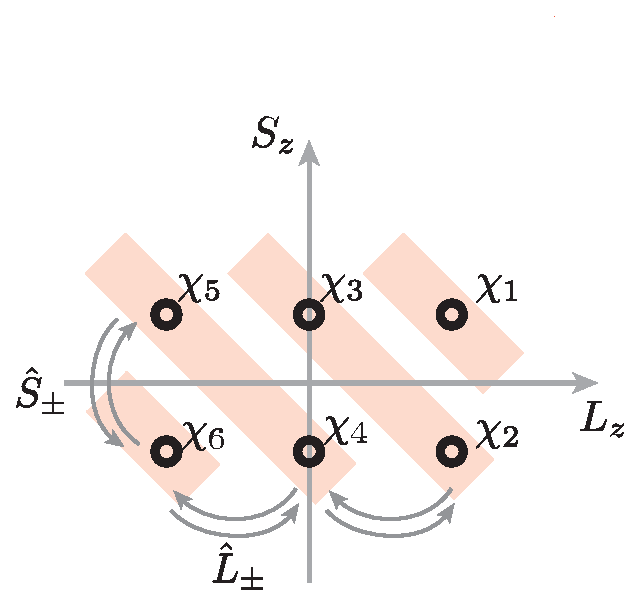
\includegraphics[width=0.4\textwidth]{pic/ls_couple.eps}
\end{figure}
\begin{enumerate}[listparindent=\parindent]
    \item 将$\hL_x=\frac{1}{2}(\hL_++\hL_-)$, $\hL_y=\frac{1}{2\im}(\hL_+-\hL_-)$代入,$\hS_x,\,\hS_y$同理,有
    \[\hat{\vec{L}}\bcdot\hat{\vec{S}}=\frac{1}{4}(\hL_++\hL_-)(\hS_++\hS_-)-\frac{1}{4}(\hL_+-\hL_-)(\hS_+-\hS_-)+\hL_z\hS_z = \frac{1}{2}(\hL_+\hS_-+\hL_-\hS_+)+\hL_z\hS_z\]
    证毕。
    
    \item 分析上问$\hat{\vec{L}}\bcdot\hat{\vec{S}}$的结果,发现若将它作用在非耦合表象的本征态$\ket{L_z,S_z}$(也即图中的每个圆点)上,结果中只会有$\ket{L_z+1,\,S_z-1}$, $\ket{L_z-1,\,S_z+1}$, $\ket{L_z,\,S_z}$这三种成分,也即不会脱离每条浅红色的区域。这是显然的,因为$\hat{\vec{L}}\bcdot\hat{\vec{S}}$与$\hat{J}_z=\hL_z+\hS_z$对易,故不会改变$J_z$的值。考虑到升降算符的作用效果为
    \[\hL_+\ket{-1,S_z}=\sqrt{2}\hbar\ket{0,S_z},\quad\hL_+\ket{0,S_z}=\sqrt{2}\hbar\ket{1,S_z}\]
    \[\hS_+\ket{L_z,-\tfrac{1}{2}}=\hbar\ket{L_z,\tfrac{1}{2}}\]
    将
    \[\hH = \frac{\varepsilon}{\hbar}(\hL_z+2\hS_z)+\frac{w}{\hbar^2}(\hL_+\hS_-+\hL_-\hS_+)+\frac{2w}{\hbar^2}\,\hL_z\hS_z\]
    分别作用到$\chi_1$到$\chi_6$上,可以得到
    \[\begin{cases}
    \hH\chi_1 = \varepsilon(1+2\cdot\frac{1}{2})\,\chi_1+2w\cdot1\cdot\frac{1}{2}\,\chi_1=(2\varepsilon+w)\,\chi_1\\
    \hH\chi_6 =\varepsilon(-1-2\cdot\frac{1}{2})\,\chi_6+2w\cdot(-1)\cdot\qty(-\frac{1}{2})\,\chi_6=(-2\varepsilon+w)\,\chi_6\\
    \hH\chi_2 =\varepsilon(1-2\cdot\frac{1}{2})\,\chi_2+\sqrt{2}w\,\chi_3+2w\cdot1\cdot\qty(-\frac{1}{2})\,\chi_2=-w\,\chi_2+\sqrt{2}w\,\chi_3\\
    \hH\chi_3 =\varepsilon(0+2\cdot\frac{1}{2})\,\chi_3+\sqrt{2}w\,\chi_2+2w\cdot0\cdot\frac{1}{2}\,\chi_3=\sqrt{2}w\,\chi_2+\varepsilon\,\chi_3\\
    \hH\chi_4 =\varepsilon(0-2\cdot\frac{1}{2})\,\chi_4+\sqrt{2}w\,\chi_5+2w\cdot0\cdot\qty(-\frac{1}{2})\,\chi_2=-\varepsilon\,\chi_4+\sqrt{2}w\,\chi_5\\
    \hH\chi_5 =\varepsilon(-1+2\cdot\frac{1}{2})\,\chi_5+\sqrt{2}w\,\chi_4+2w\cdot(-1)\cdot\frac{1}{2}\,\chi_5=\sqrt{2}w\,\chi_4-w\,\chi_5
    \end{cases}\]
    核对以上结果即可得到$c_{ij}$。
    \item 以$(\chi_1,\chi_2,\chi_3,\chi_4,\chi_5,\chi_6)$为基底写出$\hH$矩阵形式,由(b)知它在$(\chi_1)$, $(\chi_6)$, $(\chi_2,\chi_3)$, $(\chi_4,\chi_5)$上是块对角化的。作用在$\chi_1$上本征值为$2\varepsilon+w$;在$\chi_6$上本征值为$-2\varepsilon+w$。
    
    在$(\chi_2,\chi_3)$上局域矩阵为
    \[H_{23} = \mqty(-w&\sqrt{2}w\\\sqrt{2}w&\varepsilon),\]
    对角化$\abs{H_{23}-\lambda I}=(-w-\lambda)(\varepsilon-w)-2w^2=0$, 得到
    \[\lambda = \frac{-w+\varepsilon \pm\sqrt{9w^2+2w\varepsilon+\varepsilon^2}}{2}\]
    在$\varepsilon\ll w$时近似为$\lambda\approx\frac{1}{2}(-w+\varepsilon\pm 3w(1+\frac{\varepsilon}{9w}))=w+\frac{2}{3}\varepsilon$或$-2w+\frac{1}{3}\varepsilon$,在$\varepsilon\gg w$时近似为
    $\lambda\approx\frac{1}{2}(\varepsilon-w\pm\varepsilon(1+\frac{w}{\varepsilon}))=\varepsilon$或$-w$。
    
    在$(\chi_4,\chi_5)$上局域矩阵为
    \[H_{45} = \mqty(-\varepsilon&\sqrt{2}w\\\sqrt{2}w&-w),\]
    对角化$\abs{H_{45}-\lambda I}=(-\varepsilon-w)(-w-\lambda)-2w^2=0$, 得到
    \[\lambda = \frac{-w-\varepsilon \pm\sqrt{9w^2-2w\varepsilon+\varepsilon^2}}{2}\]
    在$\varepsilon\ll w$时近似为$\lambda\approx\frac{1}{2}(-w-\varepsilon\pm 3w(1-\frac{\varepsilon}{9w}))=w-\frac{2}{3}\varepsilon$或$-2w-\frac{1}{3}\varepsilon$,在$\varepsilon\gg w$时近似为
    $\lambda\approx\frac{1}{2}(-\varepsilon-w\pm\varepsilon(1-\frac{w}{\varepsilon}))=-w$或$-\varepsilon$。
    
    综上,在$\varepsilon\ll w$时,本征值为$w\pm2\varepsilon$, $w\pm\frac{2}{3}\varepsilon$, $-2w\pm\frac{1}{3}\varepsilon$;在$\varepsilon\gg w$时,本征值为$2\varepsilon+w$, $\varepsilon$, $-w$, $-w$, $-\varepsilon$, $-2\varepsilon+w$.
\end{enumerate}
\end{enumerate}
